\documentclass[11pt,a4paper]{article}
\usepackage[hyperref]{acl2017}
\usepackage{times}
\usepackage{svg}
\usepackage{url}
\usepackage{latexsym}
\usepackage{graphicx}
\usepackage{hyperref}
\usepackage{enumitem}
\usepackage{sidecap}
\usepackage{amsmath}
\usepackage[hang,flushmargin]{footmisc}
%\sidecaptionvpos{figure}{c}
\setenumerate{label=(\roman*),itemsep=1pt,topsep=1pt}
\usepackage{lipsum}

\let\OLDthebibliography\thebibliography
\renewcommand\thebibliography[1]{
  \OLDthebibliography{#1}
  \setlength{\parskip}{0pt}
  \setlength{\itemsep}{0pt plus 0.3ex}
}
%\usepackage[font=scriptsize,labelfont=bf]{caption}

%\setlength\titlebox{5cm}

% You can expand the titlebox if you need extra space
% to show all the authors. Please do not make the titlebox
% smaller than 5cm (the original size); we will check this
% in the camera-ready version and ask you to change it back.


\title{Scattertext: a Browser-Based Tool for Visualizing how Corpora Differ}

\author{Jason S. Kessler \\
  CDK Global \\
  {\tt jason.kessler@gmail.com}  \\}

\date{}

\begin{document}
\maketitle
\begin{abstract}
This paper presents Scattertext, an open source tool for visualizing linguistic variation between document categories in a language-independent way.  It is built around a novel, term-frequency based scatter-plot, where points representing thousands of words and phrases plotted, and hundreds of which are legibly labeled.  This comprehensive, legible labeling of Scattertext is an advancement from previous work in word plotting where it was impossible to label or distinguish more than a couple dozen labels.  Scattertext also lends itself to query-based visualization of how terms with similar embeddings differ between document categories.
\end{abstract}

\section{Introduction}
Finding words and phrases that discriminate categories of text is a common application of statistical NLP. For example, finding words that are most strongly characteristic of a political party in congressional speeches can help political scientist identify means of partisan framing \cite{monroe08,grimmer2010}, identifying differences in word usage between male and female characters in films can highlight narrative archetypes. \cite{schofield2016gender}, language use in social media can inform personality types \cite{Schwartz13}, and in understanding how customers evaluate restaurants \cite{jurafsky2014}.

While these studies all identify and rank category-discriminating words, a broad range of visualization techniques are used.  These include ranked lists of words, word clouds, word bubbles, and scatter clouds of words. 

Along these lines, this paper introduces a new interactive tool for discriminative language visualization.  Scattertext is based around a scatter-plot, in which each unigram or bigram used in either category is represented by a point. The coordinates of a point indicate how frequently the word in used in each category.  Figure \ref{scattertextmain} shows an example of a Scattertext plot comparing Republican and Democratic political speeches.  The higher up a point is on the y-axis, the more it was used by Democrats, and similarly the further right on the x-axis a point appears, the more its corresponding word was used by Republicans.  Highly associated terms fall closer to the upper-left and lower-right-hand corners of the chart, while stop words fall in the far upper right-hand corner.  Words occurring are typically omitted, but would fall closer to the lower-left-hand corner.  Using a mid 2014 15'' Macbook Pro, about 5,000 points can be displayed using this technique.

When used interactively, mousing-over a point shows the user statistics about a term's relative use in the two contrasting categories, and clicking on a term shows excerpts from convention speeches used.  

The point placement, intelligent word-labeling, and auxiliary term-lists ensure a low-whitespace, legible plot.  These are issues which have plagued other scatter-plot visualizations showing discriminative language.

In Section \ref{related}, I will examine the objectives, strengths and weaknesses various visualization techniques to identify discriminative words in categorized text.T he technical details behind Scattertext\footnote{\href{http://www.github.com/JasonKessler/scattertext}{github.com/JasonKessler/scattertext}} will be discussed in Section \ref{scattertext}. A related visualization task is identifying discriminating words that are semantically similar to a query.  For example, generating a visualizing that shows how members of opposing political parties use words that are similar to ``jobs'' or ``medicine'' differently. Scattertext's approach to this task--based in vector representations--is described in Section \ref{embeddings}.
\begin{figure*}[h!!]
  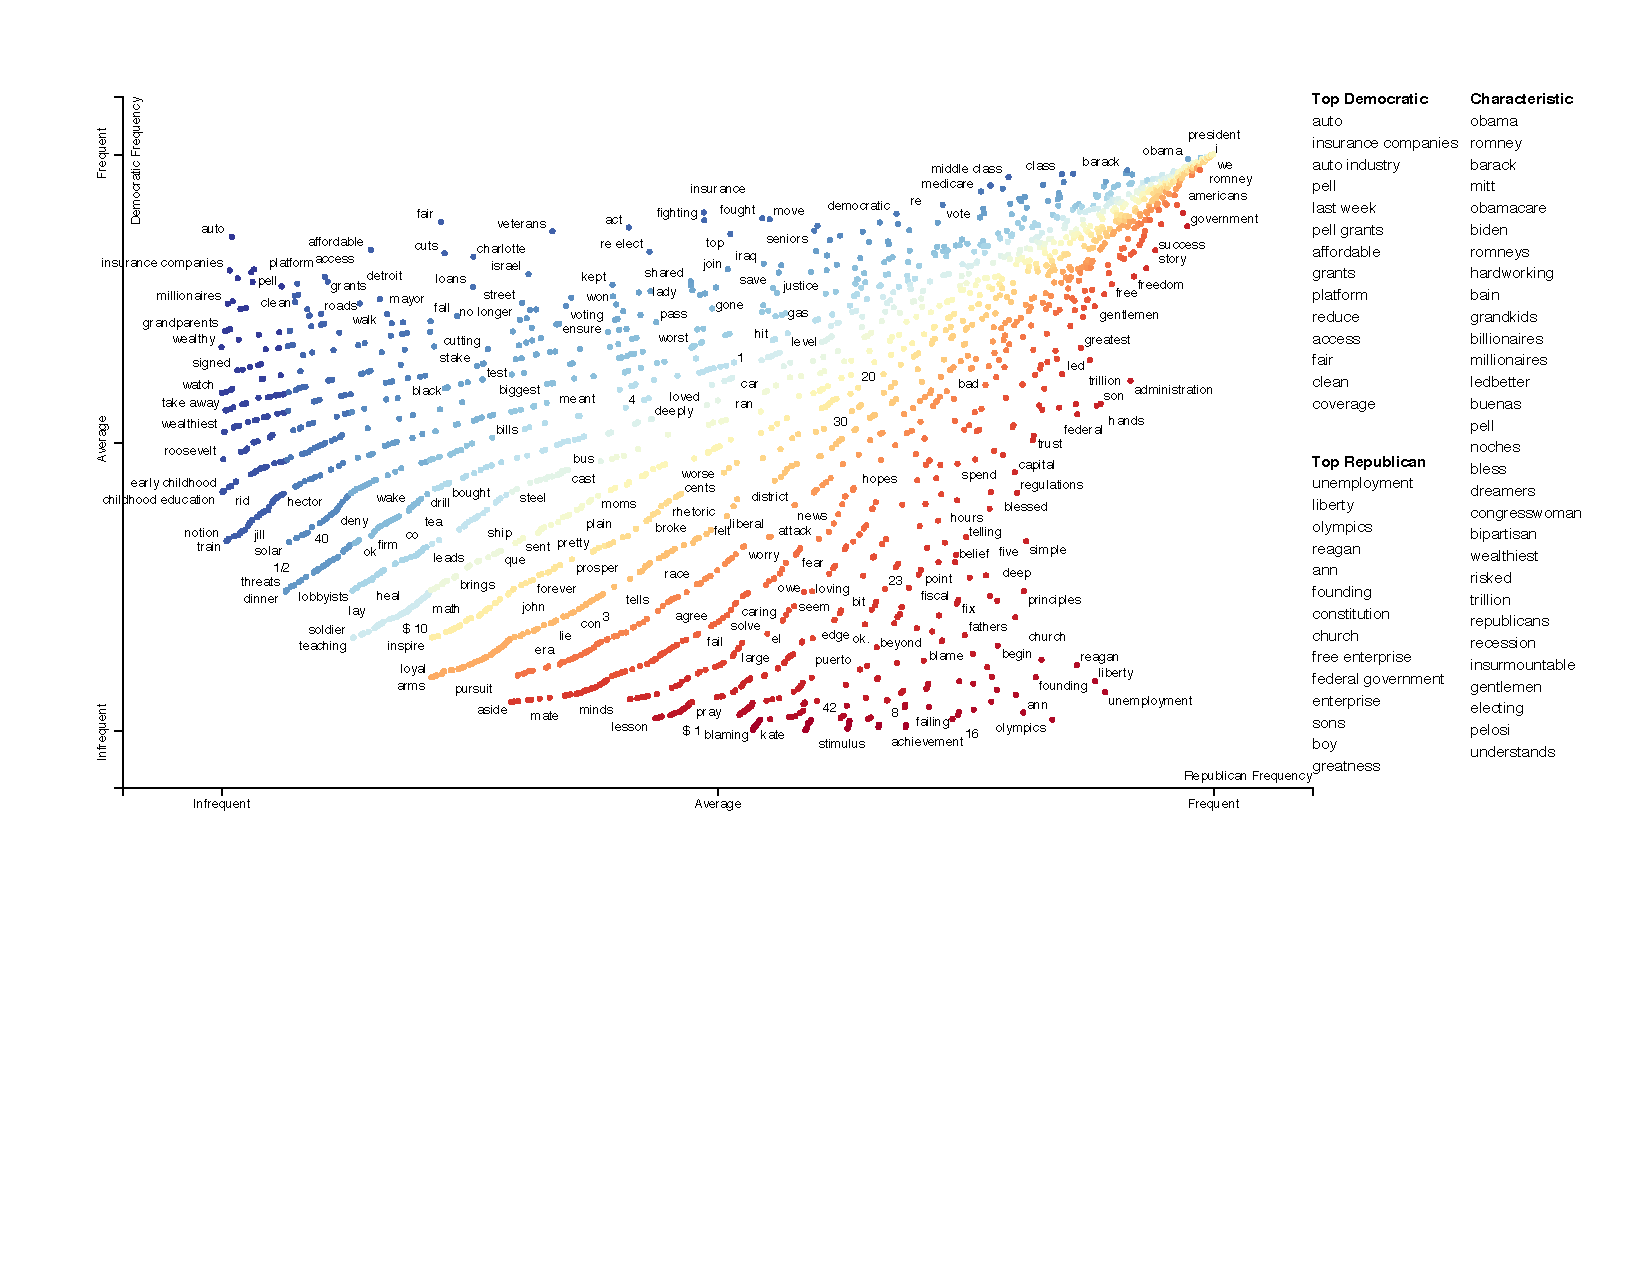
\includegraphics[width=\linewidth,scale=0.8]{primary_scattertext}
  \caption{Scattertext visualization of unigrams and bigrams used in the 2012 Political Conventions. 2,197 points are colored red or blue based on the association of their corresponding terms with Democrats or Republicans.  The most associated terms are listed under ``Top Democrat'' and ``Top Republican'' headings.}
\label{scattertextmain}
\vspace{-0.5cm}
\end{figure*}
\section{Text Visualizations}
\label{related}
The simplest visualization, a list of words ranked by their scores is easy to produce, interpret and is thus ubiquitous.  There are numerous ways of producing word scores for ranking which are throughly covered in previous work.  The reader is directed to Monroe et al. \shortcite{monroe08} for an overview of model-based term scoring algorithms.  Also of interest, Bitvai and Cohn \shortcite{Bitvai15} present a method for finding sparse words and phrase scores from a trained ANN (with bag-of-words features) and its training data. 

Regardless of how complex the calculation word scores capture a number of different measures of word-association, which can be interesting when viewed independently, instead of as part of a unitary score.  These loosely defined measures include:  \vspace{-0.1in}

\begin{description}[style=unboxed,leftmargin=0cm]
\item[Precision] A word's discriminative power regardless of its frequency.  A term that appears once in the categorized corpus will have perfect precision. This (and subsequent metrics) presuppose a balanced class distribution.  Words close to the x and y-axis in Scattertext have high precision.  \vspace{-0.1in}
\item[Recall] The frequency a word appears in a particular class, or $P(\mbox{word}|\mbox{class})$.  The variance of precision tends to decrease as recall increases.  Extremely high recall words tend to be stop-words.  High recall words occur close to the top and left sides of Scattertext plots.  \vspace{-0.1in}
\item[Non-redundancy] The level of a word's discriminative power given other words that co-occur with it.  If a word $w_a$ always co-occurs with $w_b$ and word $w_b$ has a higher precision and recall, $w_a$ would have a high level of redundancy. Measuring redundancy is non-trivial, and has traditionally been approached through l1, l2, or ElasticNet penalized logistic regression \cite{joshi2010}, as well as through other feature selection techniques.  In configurations of Scattertext such as the one shown in Figure \ref{scattertextsparse}, terms can be colored based on their regression coefficients that indicate non-redundancy.  \vspace{-0.1in}

\item[Characteristicness] How frequently the term appears in the corpus being studied relative to larger background corpus.  For example, if the categories of documents being compared are Tweets about two baseball teams and the background corpus is a sample of all of Twitter, than words like ``playoff'' or ``\#baseball'' would be characteristic of the general corpus, since they discriminate the corpus in general but not necessarily one category \cite{vennclouds}.  The terms scored highly by Formula \ref{eqn:cornerscore} are almost certainly characteristic, since they frequently appear in one category and not the other.  \vspace{-0.1in}
\end{description}

\subsection{Past Work and Design Motivation}

Complex text visualizations (i.e., not word lists) manipulate the position and appearance of words or points representing them to indicate their relative scores in these measures. For example, in Schwartz et al. \shortcite{Schwartz13}, two word clouds are given, one per each category of text being compared.  Words (which, in the study, includes 1 and selected 2 and 3-grams) are sized by their linear regression coefficients (a composite metric of precision, recall and redundancy) and colored based on how frequently words occurred.  Words selected to include in clouds had to have been used in at least 1\% of documents, and whose scores have a Bonferroni-corrected p-value of $<$0.001. Given that these words are highly correlated to their class of interest, the frequency of use is likely a good proxy for recall.

Since Shwartz et al. \shortcite{Schwartz13} create tag clouds to compare social media posts of people with one characteristic (e.g., gender or age-range) to all study participants,  characteristicness is not an interesting measure.  Coppersmith and Kelly \shortcite{vennclouds} also describe a word-cloud based visualization for discriminating terms, but intend it for categories which are both small subsets of a much larger corpus. They include a third, middle cloud for terms that appear characteristic.  The metrics used in this work require a high amount of manual tuning, which is in contrast to the other work discussed here.

Word clouds can be difficult to interpret.  It is difficult to compare the sizes of two non-horizontally adjacent words,  as well as the relative color intensities of any two words. By virtue of being larger, longer words can unintentionally appear more important.  Sizing of words can be a source of confusion when used to represent precision, since a larger word may naturally be seen as more frequent.  For these reasons, the choice was made to eschew a word-cloud like visualization.

Bostock et al. \shortcite{Bostock2012}\footnote{\href{http://www.nytimes.com/interactive/2012/09/06/us/politics/convention-word-counts.html}{nytimes.com/interactive/2012/09/06/us/politics/convention-word-counts.html}} employed an interesting, interactive word-bubble visualization for exploring different word usage among Republicans and Democrats in the 2012 American Political Conventions.  A bubble represents each term, and its size increases with its frequency of use.  It's precision is represented by it's coloring-- each bubble is colored blue and red, with the blue portion proportionally colored to a term's.  Terms were manually chosen, and arranged along the x-axis based on their discriminative power. When clicked, sentences from speeches containing the word used are listed below the visualization.  This bubble approach to word clouds inspired Nelson et al. \shortcite{Nelson2015}.

The dataset used in Bostock et al. \shortcite{Bostock2012}, consisting of 123 speeches by Democrats (76,864 words) and 66 by Republicans (58,138 words), is used to demonstrate the capabilities of Scattertext.  

\subsection{Scatter-plot visualizations}

\begin{figure}[h] 
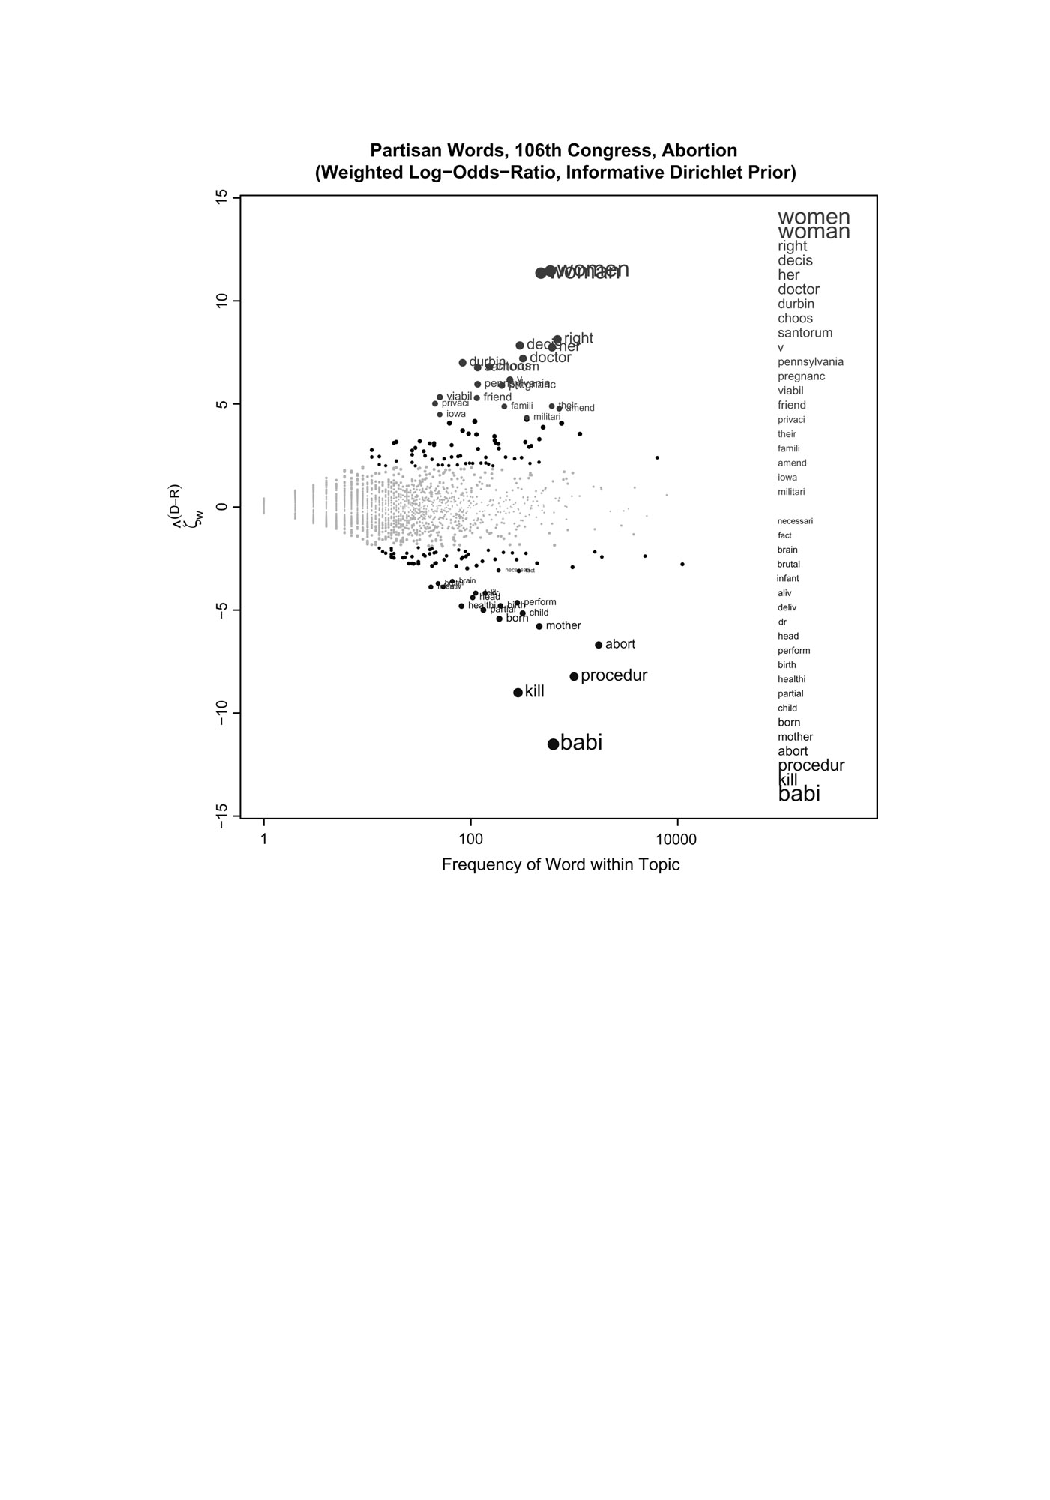
\includegraphics[width=\columnwidth]{monroefull}
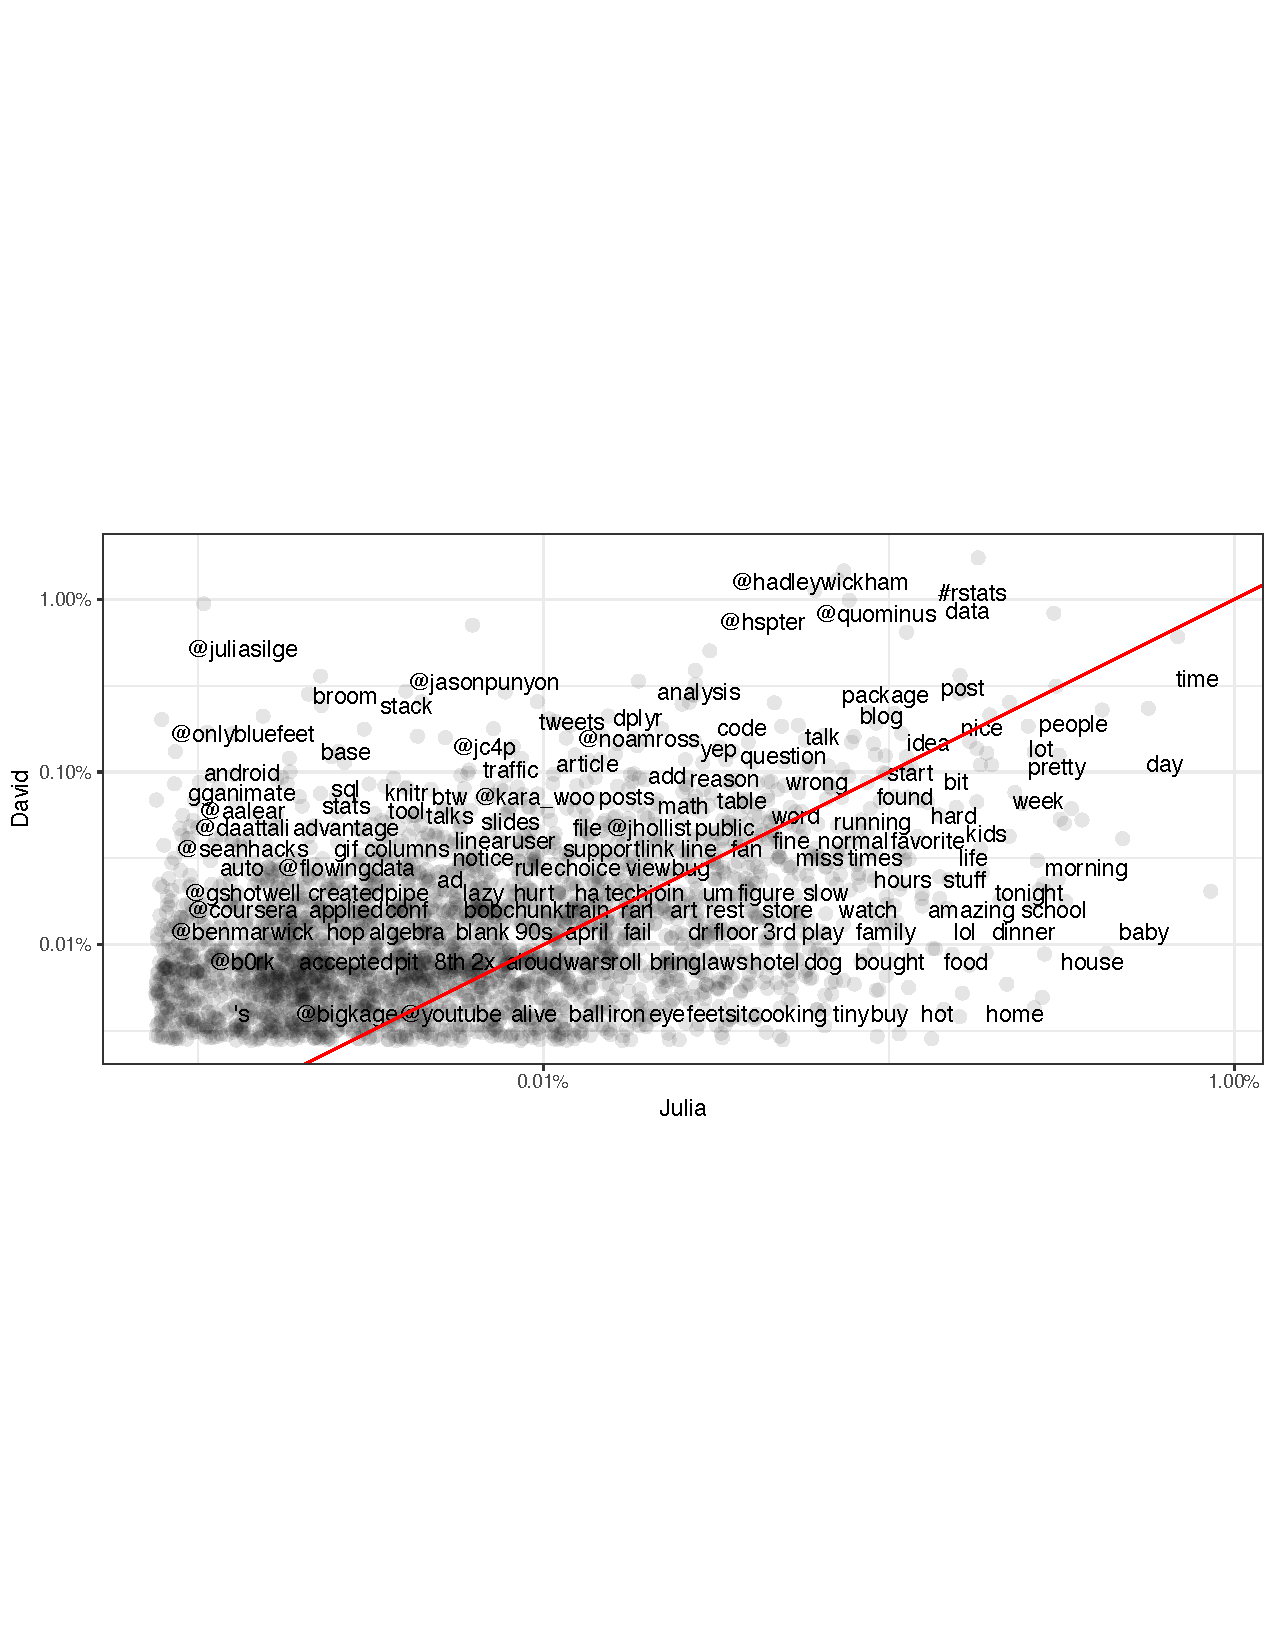
\includegraphics[width=\columnwidth]{tidytext}
\vspace{-0.8cm}
\caption{A sample of existing scatter-plot visualizations. MCQ's pref is at the top. Tidytext (Silge and Robinson, 2016) is below.} 
% Flawed solutions to the label-overlap problem: labeling points to the left of the graph \cite{schofield2016gender} (top) and non-overlapping labels of jittered points \cite{tidytext}.
\vspace{-0.5cm}
\label{scatters}
\end{figure}

Monroe et al. \shortcite{monroe08} present a visualization to illustrate the use of their proposed word score, log-odds-ratio with an informative Dirichlet prior (top of Figure \ref{scatters})  This visualization plots word-representing points along two axes.  The x-axis is log$_{10}$ recall, while the y-axis is the difference in their z-scores of their word scores.  Points with a z-score difference below 1.96 are grayed-out, while the top and bottom 20 are labeled, both by each point and on the right-hand side.  The side-labeling is necessary because labels are permitted to overlap, hindering their on-plot readability.  The sizes of points and labels are increased  proportional to the word score. This word score encompasses precision, recall, and characteristicness, since it penalizes scores of terms used more frequently in the background corpus. 

Monroe et al. \shortcite{monroe08} used this family of plot to illustrate the different profiles of various scoring techniques introduced in the paper, but the small number of points which are possible to label limit its utility for in-depth corpus analysis.  

Schofield and Mehr \shortcite{schofield2016gender} use essentially the same visualization, but plot over 100 corresponding n-grams next to an unlabeled frequency/z-score plot.  While this is appropriate for publication, displaying associated terms and the shape of the score distribution, it is impossible to align all but the highest scoring points to their labels. 

The tidytext R-package \cite{tidytext} documentation includes a non-interactive ggplot2-based \cite{ggplot2} scatter plot that is very similar to Scattertext.   The x and y-axes both, like in Scattertext, correspond to word frequencies in the two contrasting categories, with jitter added.   In the example in Figure \ref{scatters} (bottom), the contrasting categories are tweets from two different accounts.  The red diagonal line separates words with a based on their odds-ratio.  Note that much more of the chart is used by Monroe et al., 

Despite that the labels in tidytext do not overlap each other (in contrast to Monroe et al.) they do overlap points.  The points' semi-transparency makes labels in less-dense areas legible, the dense interior of the chart is nearly illegible.  Moreover, this can 

Figure 3 shows what such a plot may look like if no jitter were applied.  Words appear with the same frequency in both categories all become stacked atop each other, however this provides more interior space for labeling. 
\begin{figure}[h]
\vspace{-.25cm}
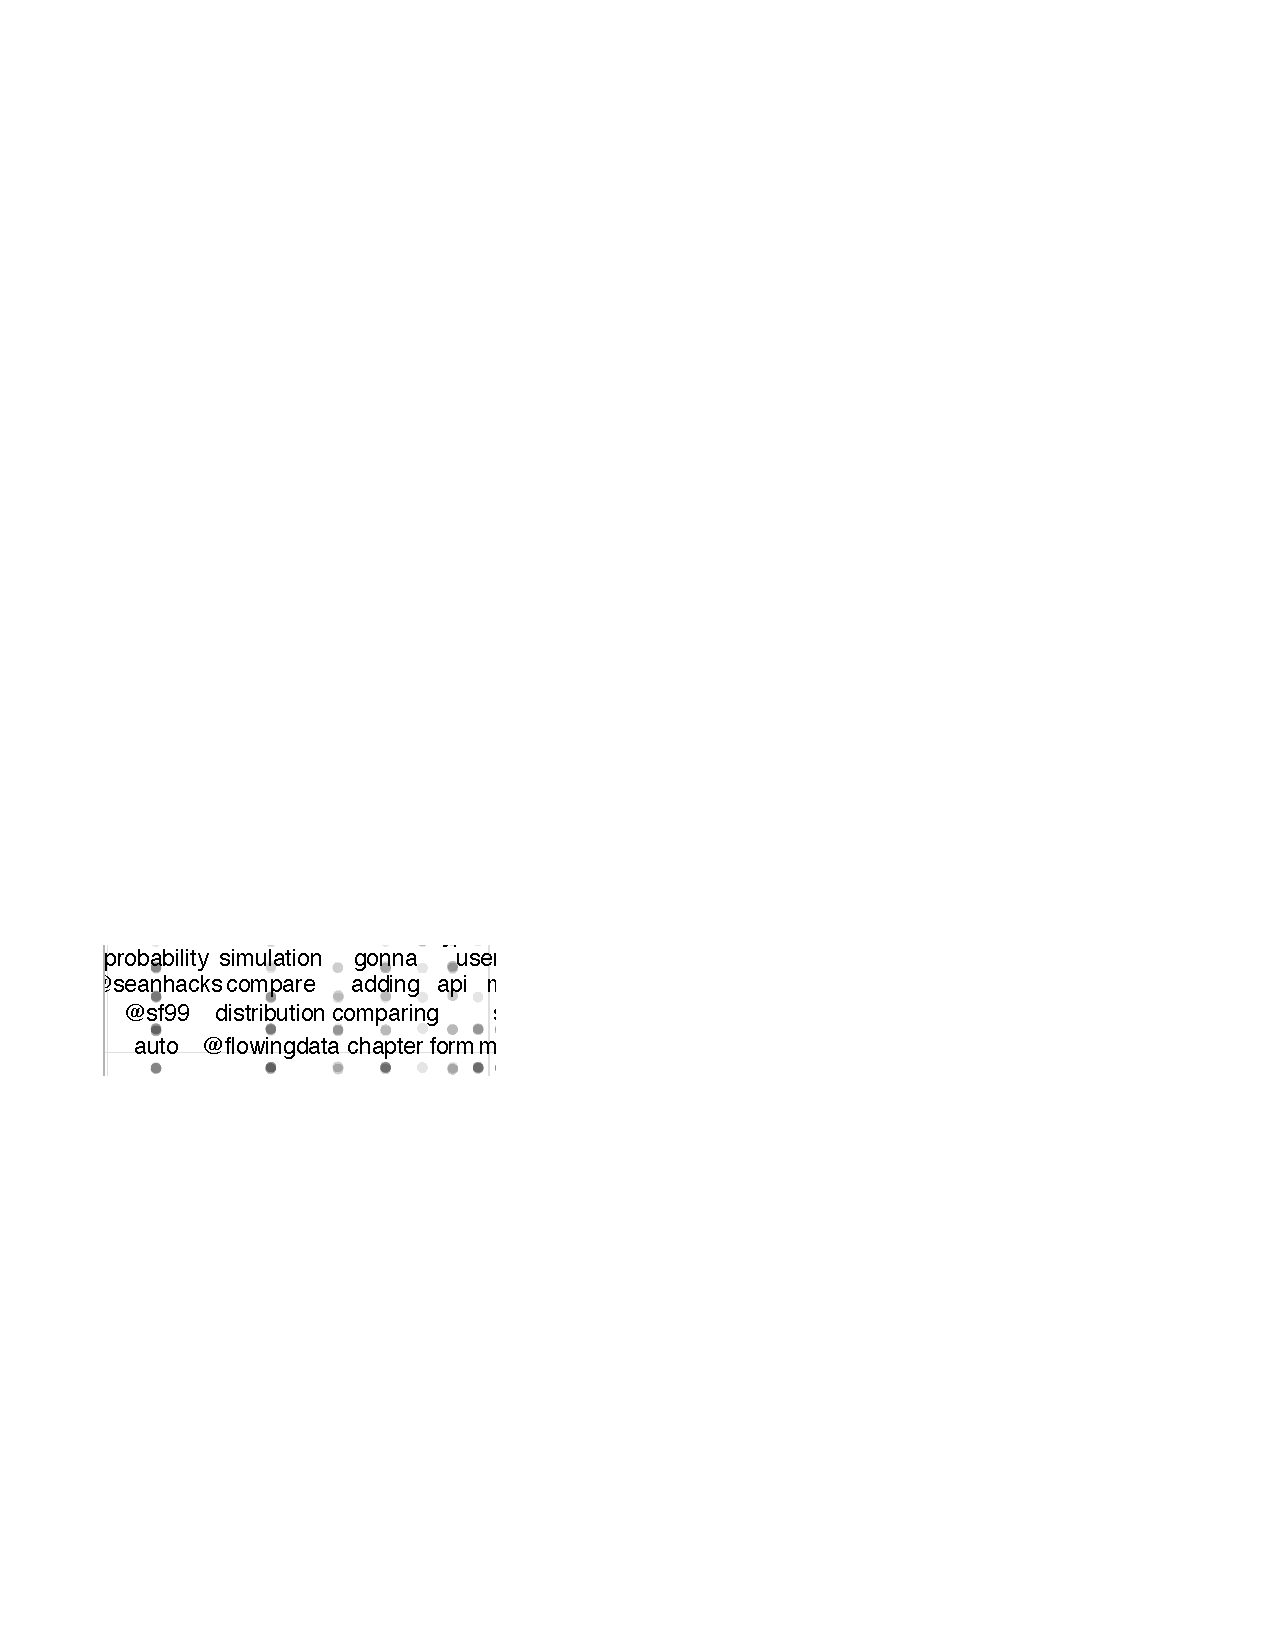
\includegraphics[width=\columnwidth]{tidytext_horiz}
\caption{A small excerpt from an un-jittered version at the bottom of Figure 2.  The dark, opaque points indicate stacks of points.}
\label{nojitterfig}
\vspace{-.25cm}
\end{figure}
The next section presents Scattertext and how its approach to word ordering solves the problems discussed above.

It should be noted this type of visualization may have first been introduced in Rudder \shortcite{Rudder2014}.
\section{Scattertext}
\label{scattertext}
Scattertext builds on tinytext and Rudder \shortcite{Rudder2014}.  It plots a set of unigrams and bigrams (we will refer to these to as ``terms'') found in a corpus documents assigned to one of two categories on a two-dimensional scatter-plot.  

In the following notation, user-supplied parameters are in bold typeface. 

Consider a corpus of documents $C$ with disjoint subsets $A$ and $B$ s.t. $A \cup B \equiv C$. Let $\phi^T$ be the number of times term $t$ occurs in $C$, $\phi^{T}(t,A)$ be the the number of times $t$ occurs in $A$. Let $\phi^{D}(t,\ldots)$ refer to the number of documents containing $t$.  Let $t_{ij}$ be the $j$th word in term $t_i$.  In practice, $j \in \{1,2\}$.   Whether $\phi^T$ or $\phi^D$ is used in formulas described below is a parameter \mbox{\boldmath$\phi$}.  Let
\begin{equation}
\vspace{-.2cm}
Pr[t_i] = \frac{\mbox{\boldmath$\phi$}(t_i)}{\sum_{t \in C\wedge|t|\equiv|t_i|} \mbox{\boldmath$\phi$}(t)}.
\vspace{-.1cm}
\end{equation}
The construction of the set of terms included in the visualization $V$ is a two-step process. Terms must occur at least \mbox{\boldmath$m$} times, and if bigrams, appear to be phrases.  In order to keep the approach language neutral, we follow Schartz et al. \shortcite{Schwartz13}, and use a pointwise mutual information score to filter out bigrams that do not occur far more frequently that would be expected.  Let
\begin{equation}
\vspace{-.2cm}
PMI(t_i) = \log \frac{Pr[t_i]}{\prod_{t_{ij}\in t_i{Pr[T_{ij}]}}}.
\vspace{-.1cm}
\end{equation}
The minimum $PMI$ accepted is \mbox{\boldmath$p$}. Now, we can define $V$ as 
\begin{equation}
\{t|\mbox{\boldmath$\phi$}(t)<\mbox{\boldmath$m$} \wedge (|t| \equiv 1 \vee PMI(t) > \mbox{\boldmath$p$}\}
\end{equation}
Let a term $t$'s coordinates on the scatter-plot be $(x^{A}_{t}, x^{B}_t)$, where $A$ and $B$ are the two document categories. Although $x^{K}_t$ is proportional to $\mbox{\boldmath$\phi$}(t,K)$, many $t$ will have identical $\mbox{\boldmath$\phi$}(t,K)$ values.  To break ties the word that appears last alphabeically will have a larger $x^{K}_t$.

We define $r^{K}_t$ s.t. $t \in V$ and $K \in \{A,B\}$ as the ranks of $\mbox{\boldmath$\phi$}(t,K)$, sorted in ascending order, where ties are broken by terms' alphabetical order.  This allows us to define \vspace{-.2cm}
\begin{equation}
\vspace{-.2cm}
x^{K}_t = \frac{r^{K}_t}{\arg\!\max r^{K}}
\end{equation}
This limits $x$ values to $[0,1]$, ensuring both axes are scaled identically.  This keeps the chart from becoming lopsided toward the corpus that had a larger number of terms. 

\textbf{Breaking ties alphabetically is a simple but important alternative to jitter.} While jitter (i.e., randomly perturbing $x_{t}^{A}$ and $x_{t}^{B}$) breaks up the stacked points shown in Figure 3, it eliminates empty space to legibly label points, and can make it seem like identically frequent points are closer to an upper-left or lower right corner.  Alphabetic tie breaking makes identical adjustments to both axes, leading to the horizontal (lower-left to upper-right) alignments of identically frequent points.  This angle does not cause one point to be substantially closer to either of the category-associated corners (the upper-left and lower-right). 

These alignments provide two advantages. First, they open up point-free tracts in the center of the chart which allow for unobstructed interior labels. Second, the align points in a way that its easy to hover a mouse over all of them, to indicate what term they correspond to, and to see be clicked to see excerpts of that term.

Rudder \shortcite{Rudder2014} observed terms closer to the lower-right corner were used frequently in $A$ and infrequently in $B$, indicating they have both high recall and precision wrt category $A$.  Symmetrically, the same relationship exists for $B$ and and the upper-right corner.  We can formalize this score between a point's coordinates and it's respective corner.  This intuition is represented by a score function $s_K(t)$ ($K\in\{A,B\}$ and $t\in V$) where
\vspace{-.3cm}
\begin{equation}
s_K(t)= 
\begin{cases} \|\langle 1-x_{t}^{A}, x_{t}^{B}\rangle\| & \text{if $K=A$,}
\\
\|\langle x_{t}^{A}, 1-x_{t}^{B}\rangle\| &\text{if $K=B$}
\end{cases}.
  \label{eqn:cornerscore}
\end{equation}

Labels are added to points in such a way as to not overlap a point or another label.  The process consists of greedily attempting to label each $t$'s point, starting with those with highest $s$ regardless of category and continuing in order of score.  12 locations around each point are tested for labeling, and if one is available, its used and the next point is examined.  An optimized data structure automatically constructed using Cozy \cite{cozy} holds the locations of points and labels. 

The top scoring terms in classes $B$ and $A$ (in Figure \ref{scattertextmain}, these are Democrats and Republicans) are listed to the left of the chart.  Hovering each labeled term (regardless of where it is on the visualization) highlights the point and gives statistics about the term.  

Points are colored based on their based on $s$.  Those corresponding to terms with a high $s_B$ colored in progressively darker shades of blue, whiles those with a higher $s_A$ are colored in progressively darker shades of red.  When both scores are about equal, the point colors become more yellow, which creates a visual divider between the two classes.   The colors are provided by D3's ``RdYlBu'' diverging-color scheme from Harrower and Brewer \cite{colorbrewer} via d3 \cite{d3}.

Other point colors (and scorings) can be used.  For example, Figure \ref{scattertextsparse} shows regression coefficients of an $\ell$1 penalized logistic regression classifier on $V$ features using document categories as labels.  Scattertext, in this example, is set to color 0 coefficients light gray.  The highly predictive words deemed redundant but still having high recall and low visible are visible in.  See below\footnote{
\href{https://jasonkessler.github.io/sparseviz.html}{jasonkessler.github.io/sparseviz.html}} for an interactive version

\begin{figure}[h]
  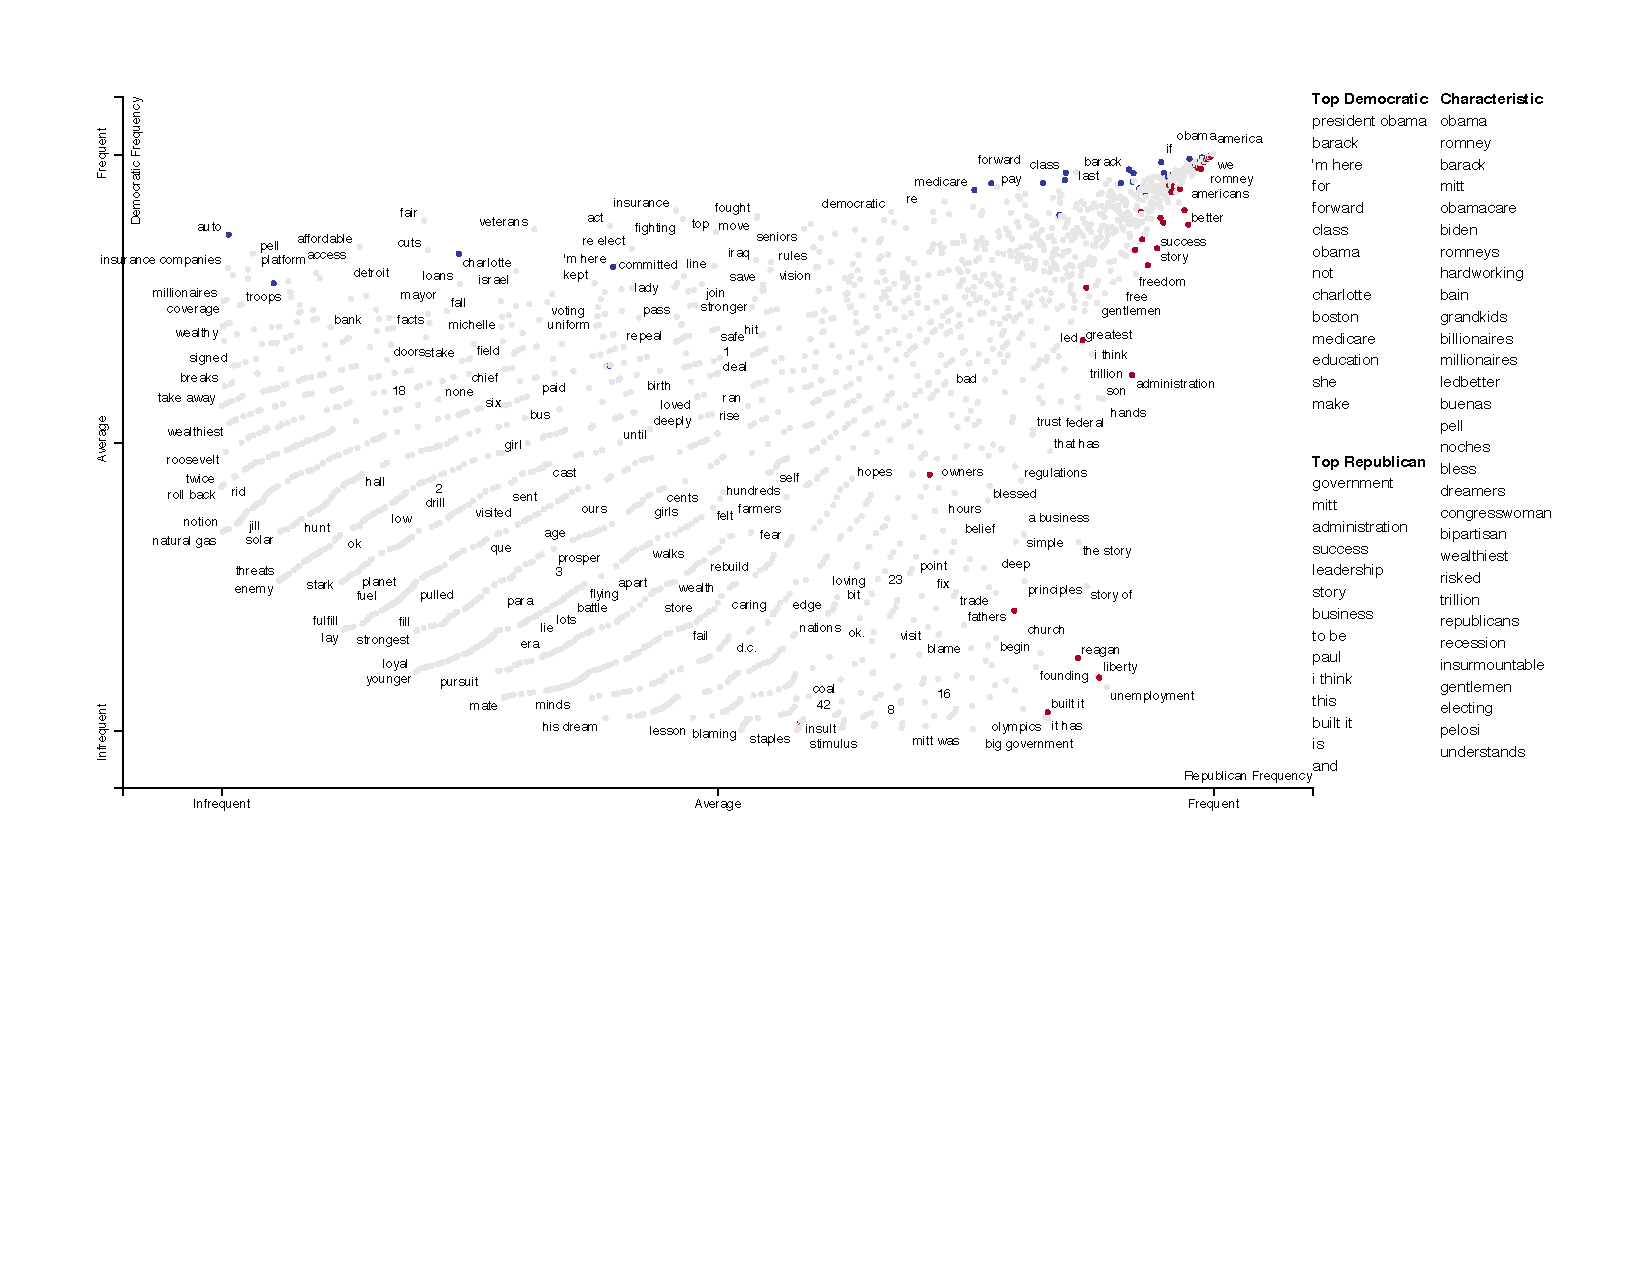
\includegraphics[width=\linewidth]{sparse_scattertext}
  \caption{Points are colored using feature weights from $\ell$1 penalized logistic regression.  Grey points have zero-weights.}
  \label{scattertextsparse}
\end{figure}

\vspace{-.25cm}
\section{Visualizing Concepts via Embeddings}
\label{embeddings}

Suppose you would like to see how see how presidential candidates used language relating to a word like ``job'', ``healthcare'', or ``military'' in American presidential convention speeches.   Figure \ref{scattertextembeddings} shows, in our running example, how Democrats and Republicans speak differently about the concept ``jobs''.  

There has been much work in visualizing word embeddings\footnote{E.g., \href{http://projector.tensorflow.org/}{projector.tensorflow.org}}, none to the knowledge of this author has focused on visualizing category-discriminating embeddings.

In this configuration of Scattertext, words are colored by their similarity to a query phrase.  This is done using spaCy\footnote{\href{https://spacy.io/}{spacy.io}}-provided GloVe \cite{glove} word vectors (trained on the Common Crawl corpus).  Similarity is measured via cosine distance between the mean embeddings of each word in the query phrase each term embedding (mean embeddings are taken from bigram terms).  

\begin{figure}[h]
  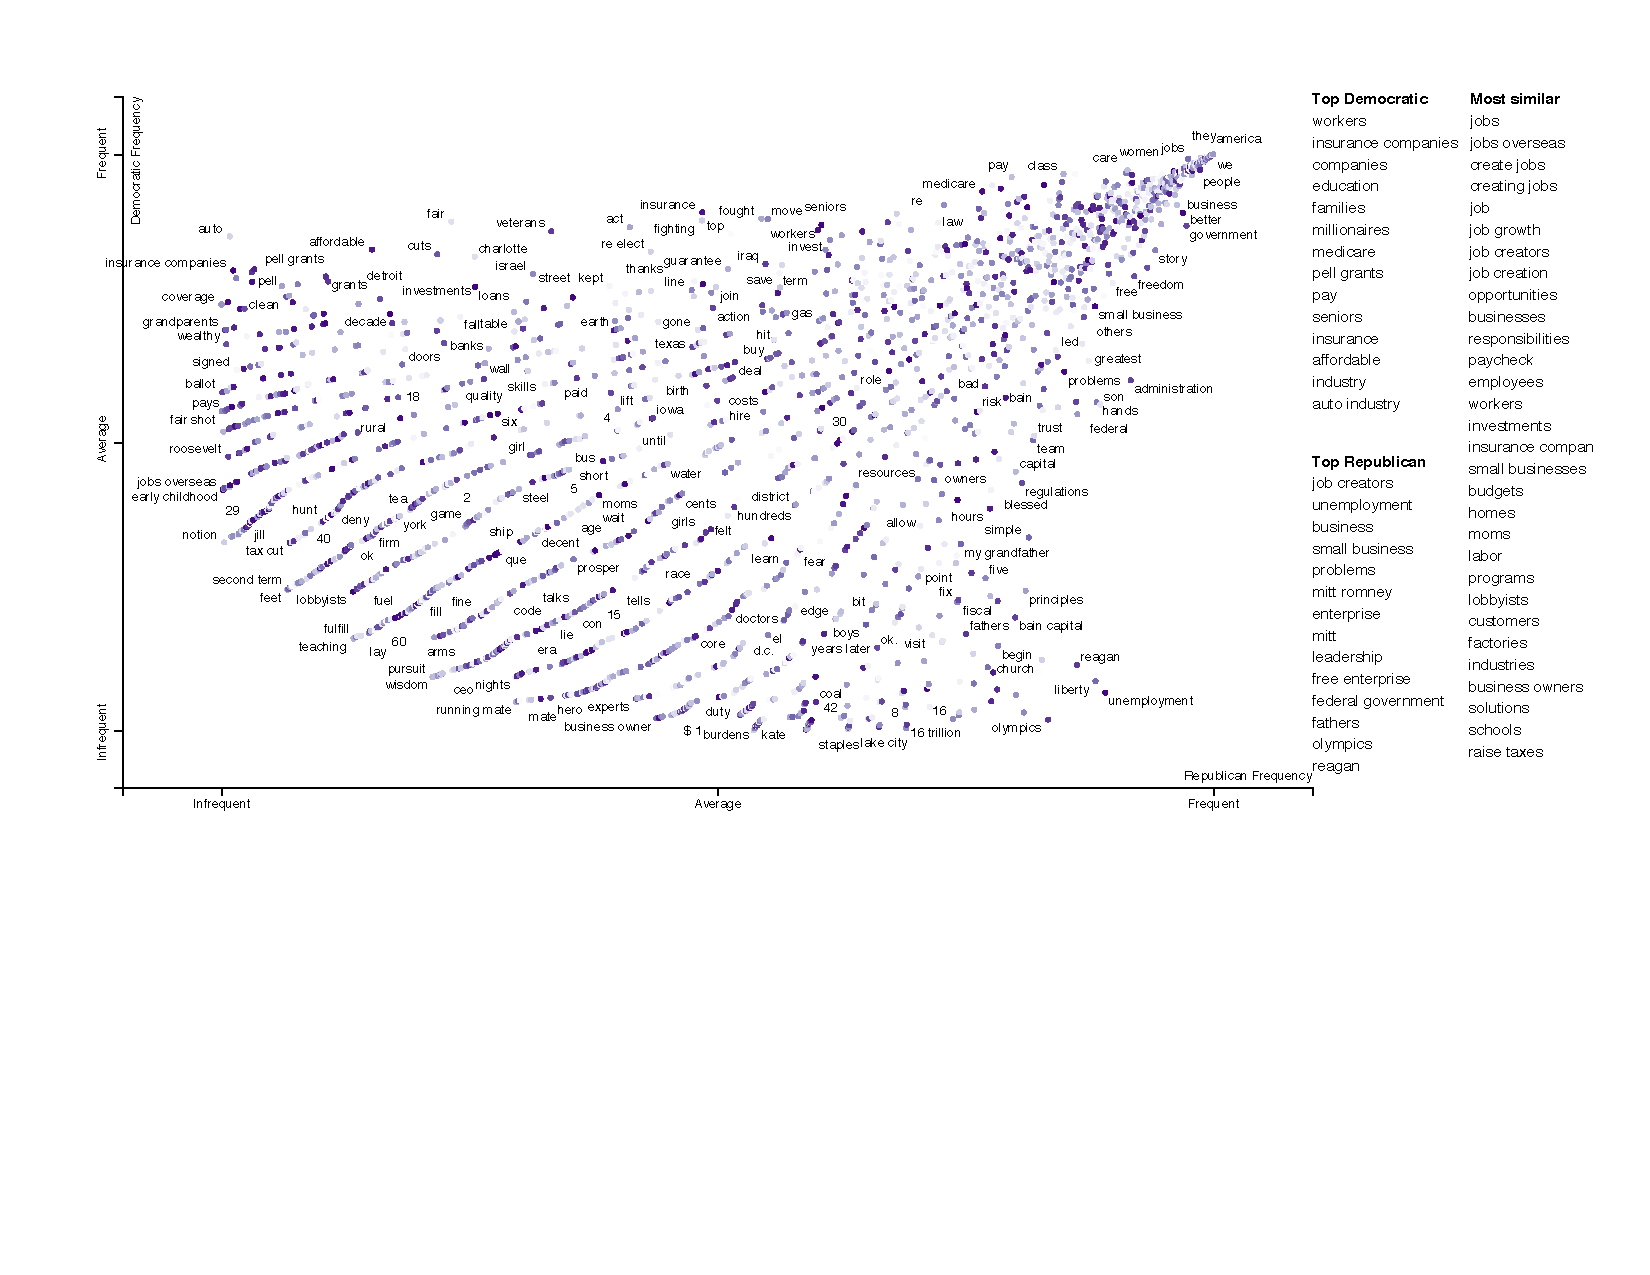
\includegraphics[width=\linewidth]{similarity_scattertext}
  \caption{Words and phrases that are semantically similar to the word ``jobs`` are colored darker, and general and category-specific related terms are listed to the right\footnote{Interactive version: \href{https://jasonkessler.github.io/demosim.html}{jasonkessler.github.io/demosim.html}}.}
  \label{scattertextembeddings}
\vspace{-.2cm}
\end{figure}
The calculation of the most similar terms associated with each category is a simple heuristic which appears to work well.  For each category, a set of associated terms is found and the most similar terms to the query from that listed as ``Top'' terms to the right of the scatter-plot.  The associated terms are identified through having p-values $<$0.05, using Monroe et al. \shortcite{monroe08}'s difference in weighted log-odds-ratio with an uninformative Dirichlet prior.  Three model-based, regularized version of log-odds-ratio are introduced in Monroe et al.  The two preferred models rely on the presence of an in-domain background corpus of sufficient size to penalize common terms, and only unigrams are used in their study.  

The remaining function relies on a the hyperparameter \mbox{\boldmath$\alpha$} to be passed to the Dirichlet prior.  \mbox{\boldmath$\alpha$} is a vector of size $|V|$, and example of Monroe et al. is followed using a uniform value of $0.01$.  Formulas (16), (18) and (22) are used to compute term z-scores, which are then converted to p-values using the Normal CDF of $\hat{\zeta}_{w}^{A-B}$, letting $y^{(K)}_{t} = \mbox{\boldmath$\phi$}(t,K)$ st ${K}\in{\{A,B\}}$ and $t\in{V}$.

As seen in Figure \ref{scattertextembeddings}, the top Republican word related to ``jobs'' is ``job creators'', while ``workers'' is the top Democratic term.

\vspace{-0.3cm}
\nocite{ggplot2}
\nocite{Rudder2014}
\nocite{tidytext}

\bibliography{kessler2017}
\bibliographystyle{acl_natbib}
\end{document}
